\documentclass[12pt, titlepage]{article}

\usepackage{booktabs}
\usepackage{tabularx}
\usepackage{amsmath}
\usepackage{siunitx}
\usepackage{float}
\usepackage{hyperref}
\hypersetup{
    colorlinks,
    citecolor=black,
    filecolor=black,
    linkcolor=red,
    urlcolor=blue
}
\usepackage{tikz}
\usepackage{pgfplots}
\pgfplotsset{compat=1.18}

\usepackage{xr,xr-hyper}
\externaldocument{../SRS/SRS}
\externaldocument{../Design/SoftArchitecture/MG}
\externaldocument{../VnVPlan/VnVPlan}

\newcommand{\rref}[1]{R\ref{#1}}
\newcommand{\nfrref}[1]{NFR\ref{#1}}
\newcommand{\mref}[1]{M\ref{#1}}
\newcommand{\tref}[1]{T\ref{#1}}

\usepackage[backend=biber,style=authoryear]{biblatex}
\addbibresource{../../refs/References.bib}

\input{../Comments}
%% Common Parts

\newcommand{\progname}{MPIR} % PUT YOUR PROGRAM NAME HERE
\newcommand{\authname}{Xunzhou (Joe) Ye} % AUTHOR NAMES

\newcommand{\matr}[1]{\mathbf{#1}}
\renewcommand{\vec}[1]{\mathbf{#1}}
\newcommand{\spann}[1]{\mathrm{span}\{#1\}}

\usepackage{hyperref}
    \hypersetup{colorlinks=true, linkcolor=blue, citecolor=blue, filecolor=blue,
                urlcolor=blue, unicode=false}
    \urlstyle{same}


\begin{document}

\title{Verification and Validation Report: \progname}
\author{\authname}
\date{\today}

\maketitle

\pagenumbering{roman}

\section{Revision History}

\begin{tabularx}{\textwidth}{p{3cm}p{2cm}X}
  \toprule {\bf Date}  & {\bf Version} & {\bf Notes}   \\
  \midrule
  \date{16 April 2025} & 1.0           & Initial draft \\
  \bottomrule
\end{tabularx}

~\newpage

\section{Symbols, Abbreviations and Acronyms}

\renewcommand{\arraystretch}{1.2}
\begin{tabular}{l l}
  \toprule
  \textbf{symbol} & \textbf{description}\\
  \midrule
  T & Test\\
  \bottomrule
\end{tabular}\\

\wss{symbols, abbreviations or acronyms -- you can reference the SRS tables if needed}

\newpage

\tableofcontents

\listoftables %if appropriate

\listoffigures %if appropriate

\newpage

\pagenumbering{arabic}

\section{Functional Requirements Evaluation}

In this section, the system tests that will be conducted are described in
detail. These tests will be used to verify the fulfillment of the functional
requirements as listed in the SRS (\cite{SRS}).

\subsection{Matrix Inputs and Outputs}

This section covers the requirement \rref{R:ex} of the SRS. This includes
essentially a ``driver'' for the solver which loads sparse matrices from a text
file in Matrix Market Exchange (.mtx) Format (\cite{noauthor_matrix_2013}) into memory,
invokes the solver interfaces, and outputs the results returned from the solver.
The tests described below will verify that such a ``driver'' is functional.

\begin{itemize}

\item[\tref{T:io}]{matrix-io}

  Output: The elements of \(\matr{A}\) matches exactly the one in the .mtx file.
  Result solution \(\vec{x}\) is of size \num{100}.

  Result: Pass
\end{itemize}

\subsection{Correctness Tests with Manufactured Solutions}
\label{sec:corr-tests-with}

This section covers one of the ways to verify the requirements \rref{R:Axb} and
\rref{R:MP} of the SRS. This includes tests on the accuracy of the solution from
the solver by manufacturing an exact solution \(\vec{x}_\mathrm{ref}\) to the
problem \(\matr{A}\vec{x} = \vec{b}\). This manufacturing process loosely
follows the scheme below:

\begin{enumerate}
\item \(\vec{x}_\mathrm{ref} \gets \text{some random vector}\)
\item \(\vec{b} \gets \matr{A} \vec{x}_\mathrm{ref} \)
\item Solve \(\matr{A}\vec{x} = \vec{b}\)
\item \(e \gets \displaystyle \frac{\norm{\vec{x} - \vec{x}_\mathrm{ref}}_2}{\norm{\vec{x}_\mathrm{ref}}_2}\)
\end{enumerate}

The relative error \(e\) will be used as the accuracy metric. The values of the
manufactured reference solution \(\vec{x}_\mathrm{ref}\) in this section is
uniformly distributed in the range of \([\min(a_{i,j}), \max(a_{i,j})]\). For
the test cases in Sections~\ref{sec:corr-tests-with},
\ref{sec:corr-tests-against}, and below, the \texttt{bundle1} matrix
(\cite{m_lourakis_lourakisbundle1_2006}) from the Florida Sparse Matrix
Collection (\cite{davis_university_2011}) will be used as the input matrix
\(\matr{A}\). This matrix has a size of \(\num{10581} \times \num{10581}\) and
\num{770811} non-zeros. The estimated condition number is \num{1.3e4}.

\begin{itemize}

\item[\tref{T:gdd}:]{generated-double-double}

  Output: \(\vec{x}\) with \(e = \displaystyle \frac{\norm{\vec{x} -
      \vec{x}_\mathrm{ref}}_2}{\norm{\vec{x}_\mathrm{ref}}_2} < \num{1e-10}\)

  Result: Pass

\item[\tref{T:gsd}:]{generated-single-double}

  Output: \(\vec{x}\) with \(e = \displaystyle \frac{\norm{\vec{x} -
      \vec{x}_\mathrm{ref}}_2}{\norm{\vec{x}_\mathrm{ref}}_2} < \num{1e-10}\)

  Result: Pass

\end{itemize}

\subsection{Correctness Tests against Trusted Solvers}
\label{sec:corr-tests-against}

This section covers the other way to verify the requirements \rref{R:Axb} and
\rref{R:MP} of the SRS. This includes tests on the accuracy of the yielded
solution from the solver by comparing it to an external, trusted solver to the
problem \(\matr{A}\vec{x} = \vec{b}\). This process loosely follows the scheme
below:

\begin{enumerate}
\item \(\vec{x}_\mathrm{ref} \gets \text{solution by an external solver}\)
\item Solve \(\matr{A}\vec{x} = \vec{b}\)
\item \(e \gets \displaystyle \frac{\norm{\vec{x} - \vec{x}_\mathrm{ref}}_2}{\norm{\vec{x}_\mathrm{ref}}_2}\)
\end{enumerate}

The relative error \(e\) will be used as the accuracy metric. For the test cases
in this Section, MATLAB\textsuperscript{\textregistered} will be used as the
external reference solver.

\begin{itemize}

\item[\tref{T:exdd}:]{external-double-double}

  Output: \(\vec{x}\) with \(e = \displaystyle \frac{\norm{\vec{x} -
      \vec{x}_\mathrm{ref}}_2}{\norm{\vec{x}_\mathrm{ref}}_2} < \num{1e-10}\)

  Result: Pass

\item[\tref{T:exsd}:]{external-single-double}

  Output: \(\vec{x}\) with \(e = \displaystyle \frac{\norm{\vec{x} -
      \vec{x}_\mathrm{ref}}_2}{\norm{\vec{x}_\mathrm{ref}}_2} < \num{1e-10}\)

  Result: Pass

\end{itemize}

\section{Nonfunctional Requirements Evaluation}

\subsection{Accuracy}

The accuracy of the solver is assessed by verifying that it converges to a
solution within the user-defined tolerance \(\epsilon\). The level of accuracy
required for computational science and engineering applications will be
evaluated through the relative residual norm after convergence. The functional
tests \tref{T:gdd}, \tref{T:gsd}, \tref{T:exdd}, \tref{T:exsd} are sufficient to
verify the nonfunctional requirement \nfrref{NFR:acc} in the SRS with an
accuracy metric of \(\epsilon \approx \num{1e-10}\). Considering that the
residual precision \(u_r = \texttt{double}\), the chosen \(\epsilon \approx
\num{1e-10}\) is reasonably close to the machine epsilon in \texttt{double}
precise \(\epsilon_\mathrm{mach} \approx \num{1.1e-16}\).

\subsection{Usability}

The usability of the solver will be evaluated based on the clarity and
accessibility of its public Application Programming Interface (API). The API
should be self-contained, readable, and easy to integrate into other software as
a dependency. Usability testing will reference the user characteristics section
and include developer feedback. The following tests will be performed to verify
the nonfunctional requirement \nfrref{NFR:use} in the SRS:

\begin{itemize}

\item[\tref{T:use}:]{nfr-use}

  Output/Result: Pass

  The usability survey feedback was largely positive, highlighting the API’s
  clarity and ease of integration, with a few suggestions for expanding
  documentation and use-case coverage. See Appendix~\ref{sec:usab-surv-results} for
  a detailed report.

\end{itemize}

\subsection{Maintainability}

The maintainability test \tref{T:mt} was not executed due to the time
constraints of the project and the nature of the proposed changes. Implementing
support for an additional matrix storage format (CSR) is possible but still
requires efforts to implement. While such a change would offer a meaningful
scenario to assess maintainability, it is outside the defined scope of the
current project, which focuses on mixed-precision solver strategies for matrices
in CSC format. The maintainability test is acknowledged but deferred as future
work or as a candidate for post-project evaluation.


\subsection{Portability}

The solver should run on all actively maintained operating systems, including
Windows 10, Windows 11, Linux, and MacOS. Compatibility testing will verify that
all required functionalities work across different platforms. The following
tests will be performed to verify the nonfunctional requirement \nfrref{NFR:port}
in the SRS:

\begin{itemize}

\item[\tref{T:port}:]{nfr-port}

Output/Result: Pass, See
\href{https://github.com/yex33/MPIR/actions/workflows/ctest.yml}{CTest Github Action}.

\end{itemize}

\subsection{Performance}

To fulfill the nonfunctional requirement for performance \nfrref{NFR:perf}, a
manual benchmark test will be conducted to evaluate the solver’s runtime
efficiency when using mixed-precision arithmetic. The runtime of the functional
tests \tref{T:gdd} and \tref{T:gsd} will serve as the basis for comparing
performance between two configurations:
\begin{enumerate}
\item Mixed-precision mode: factorization in single precision, internal solves and
  residual evaluations in double precision.
\item Double-precision mode: all computations in double precision.
\end{enumerate}
Each test will be executed multiple times to account for variability and ensure
statistically stable results. This is necessary because clock-time measurements
on modern processors can be affected by factors such as CPU caching, thermal
throttling, and OS-level scheduling.

\begin{itemize}

\item[\tref{T:perf}:]{nfr-perf}

  Output/Result: The mixed-precision configuration consistently outperformed the
  full double-precision mode, achieving a 24.25\% reduction in runtime on a
  representative sparse matrix. The results meet the nonfunctional performance
  requirement outlined in \nfrref{NFR:perf}, confirming the efficiency advantage
  of the mixed-precision implementation. Test data is attached in
  Appendix~\ref{sec:perf-test-results}.

\end{itemize}

\section{Comparison to Existing Implementation}

A detailed comparison of the current implementation of the preconditioned GMRES
algorithm against the previous prototype is provided in
Appendix~\ref{sec:textttpr-comp}. The improvements made to this core algorithm
reflect a broader design philosophy adopted throughout the development of
\progname{}:

\begin{itemize}
\item A cleaner and safer C++ interface, with significantly fewer template
  parameters.
\item Use of standard containers (\texttt{std::vector}) to eliminate manual memory
  management and reduce the risk of resource leaks.
\item Decomposition of complex numerical routines into self-contained, reusable
  primitives, enhancing both readability and testability.
\item A consistent type-safety mechanism using the \texttt{Refinable} concept, replacing
  scattered manual casts.
\item Direct return of computed results, enabling more idiomatic error handling and
  seamless integration.
\end{itemize}

\section{Unit Testing}
\label{sec:unit-testing}

All tests passing. See
\href{https://github.com/yex33/MPIR/actions/workflows/ctest.yml}{CTest Github
  Action}.

\section{Changes Due to Testing}

\wss{This section should highlight how feedback from the users and from
the supervisor (when one exists) shaped the final product.  In particular
the feedback from the Rev 0 demo to the supervisor (or to potential users)
should be highlighted.}

Due to project time constraints and the scope of the current phase, no further
implementation changes were made following this round of testing.

\section{Automated Testing}

Refer to Section~\ref{sec:unit-testing}.

\section{Trace to Requirements}

\begin{table}[H]
  \centering
  \begin{tabular}{|c|c|c|c|c|c|c|c|c|}                                      \hline
                  & \rref{R:Axb} & \rref{R:MP} & \rref{R:ex} & \nfrref{NFR:acc} & \nfrref{NFR:use} & \nfrref{NFR:mt} & \nfrref{NFR:port} & \nfrref{NFR:perf} \\ \hline
    \tref{T:io}   &              &             & X           &                  &                  &                 &                   &                   \\ \hline
    \tref{T:gdd}  & X            & X           &             & X                &                  &                 &                   &                   \\ \hline
    \tref{T:gsd}  & X            & X           &             & X                &                  &                 &                   &                   \\ \hline
    \tref{T:exdd} & X            & X           &             & X                &                  &                 &                   &                   \\ \hline
    \tref{T:exsd} & X            & X           &             & X                &                  &                 &                   &                   \\ \hline
    \tref{T:use}  &              &             &             &                  & X                &                 &                   &                   \\ \hline
    \tref{T:mt}   &              &             &             &                  &                  & X               &                   &                   \\ \hline
    \tref{T:port} &              &             &             &                  &                  &                 & X                 &                   \\ \hline
    \tref{T:perf} &              &             &             &                  &                  &                 &                   & X                 \\ \hline
  \end{tabular}
  \caption{Traceability matrix showing the connections between test cases and
    requirements}
  \label{Table:T_trace}
\end{table}

\section{Trace to Modules}

No specific test case is given in Section~\ref{sec:unit-testing}, but the unit
testing strategy has been covered for each tested module.

\section{Code Coverage Metrics}

Code coverage testing was not performed in this project due to the following
considerations:

\begin{itemize}
\item Given the limited development timeline, priority was given to functional
  correctness, numerical accuracy, and performance testing—areas more critical
  for a numerical solver in a research context.
\item The primary objective of the project was to validate the correctness and
  performance of the underlying numerical methods (e.g., mixed-precision GMRES
  and iterative refinement), rather than achieving high test coverage metrics.
\item Since the solver is structured around reusable, well-scoped numerical
  routines that are individually tested with known inputs and analytical
  results, the marginal benefit of computing line or branch coverage was minimal
  compared to the effort required to instrument and interpret those metrics.
\end{itemize}
\newpage{}

\printbibliography{}

\newpage{}

\appendix{}
\addcontentsline{toc}{section}{Appendices}
\section*{Appendices}

\section{Usability Survey Results}
\label{sec:usab-surv-results}

\subsection{Summary}

A usability evaluation was conducted on the solver’s public API by three VnV
team members with experience in numerical software development. Participants
reviewed the API documentation, examined usage examples, and completed a
structured survey comparing the solver's API to Eigen's sparse solver interface.

The feedback was largely positive, highlighting the API’s clarity and ease of
integration, with a few suggestions for expanding documentation and use-case
coverage.

\subsection{Participant Summary}

\begin{tabularx}{\linewidth}{lX}
  \toprule
  \textbf{Reviewer} & \textbf{Background}                          \\
  \midrule
  Reviewer A  & MSc student, numerical linear algebra  \\
  Reviewer B  & Senior undergrad, software engineering \\
  Reviewer C  & TA, scientific computing               \\
  \bottomrule
\end{tabularx}

\subsection{Likert Scale Results}

\begin{tabularx}{\linewidth}{lcccc}
  \toprule
  \textbf{Question}                   & \textbf{Very Good} & \textbf{Good} & \textbf{Neutral} & \textbf{Poor} \\
  \midrule
  Q1. Intuitive function names  & 2            & 1       & 0          & 0       \\
  Q2. Clear documentation       & 2            & 1       & 0          & 0       \\
  Q3. Sufficient examples       & 1            & 2       & 0          & 0       \\
  Q4. Ease of setup             & 1            & 2       & 0          & 0       \\
  Q5. Quality of error messages & 1            & 2       & 0          & 0       \\
  Q7. Overall usability         & 2            & 1       & 0          & 0       \\
  Q9. Recommend API             & 2            & 1       & 0          & 0       \\
  \bottomrule
\end{tabularx}

\subsection{Open-Ended Feedback Highlights}

\begin{itemize}
  \item \textit{Q6. Encountered difficulties:}
  \begin{itemize}
    \item “It wasn't immediately clear how to switch between CSC and CSR modes.”
    \item “I expected a higher-level wrapper function that hides the solver config setup.”
  \end{itemize}
  \item \textit{Q8. Suggestions for improvement:}
  \begin{itemize}
    \item “Add more detailed documentation for return types and default configurations.”
    \item “Include an end-to-end integration example with a real-world sparse matrix.”
  \end{itemize}
\end{itemize}

\subsection{Summary Graphs}

\begin{figure}[H]
  \centering
  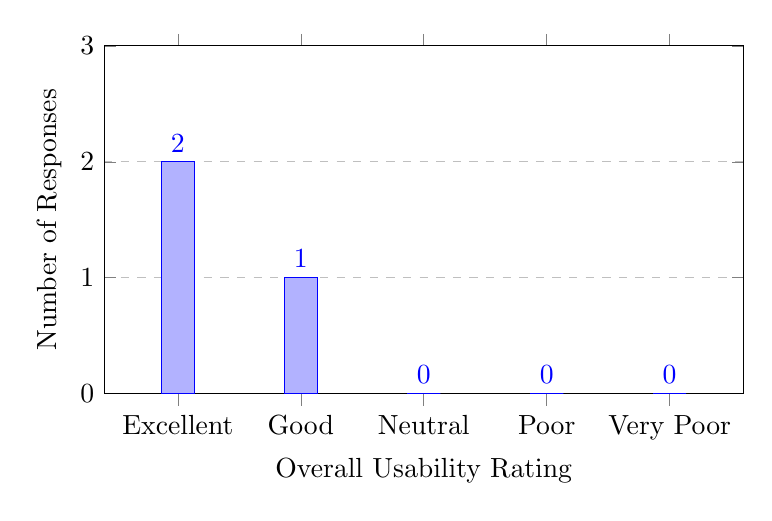
\begin{tikzpicture}
    \begin{axis}[
      ybar,
      bar width=12pt,
      width=0.8\textwidth,
      height=6cm,
      enlarge x limits=0.15,
      ylabel={Number of Responses},
      xlabel={Overall Usability Rating},
      symbolic x coords={Excellent, Good, Neutral, Poor, Very Poor},
      xtick=data,
      nodes near coords,
      ymin=0, ymax=3,
      ymajorgrids=true,
      grid style=dashed,
      ]
      \addplot coordinates {(Excellent,2) (Good,1) (Neutral,0) (Poor,0) (Very Poor,0)};
    \end{axis}
  \end{tikzpicture}
  \caption{Overall Usability Rating}
\end{figure}

\begin{figure}[H]
  \centering
  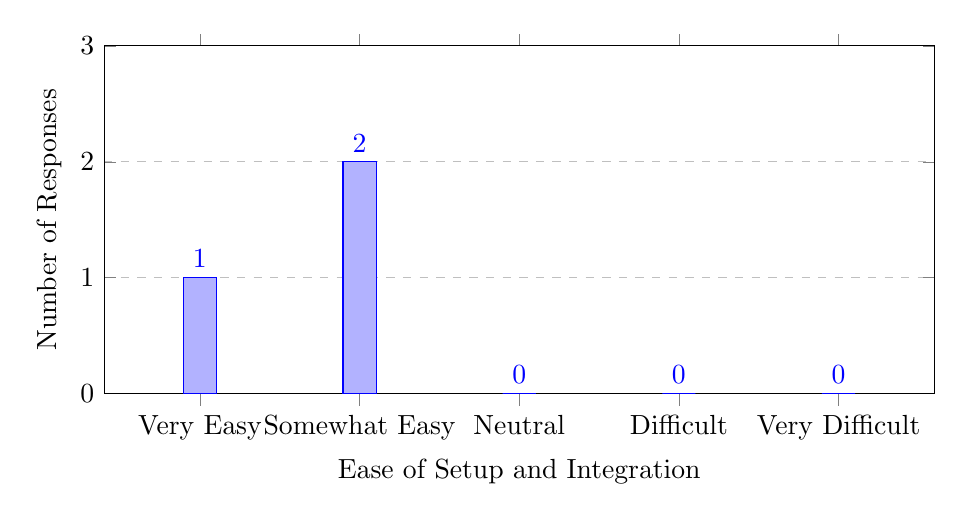
\begin{tikzpicture}
    \begin{axis}[
      ybar,
      bar width=12pt,
      width=1\textwidth,
      height=6cm,
      enlarge x limits=0.15,
      ylabel={Number of Responses},
      xlabel={Ease of Setup and Integration},
      symbolic x coords={Very Easy, Somewhat Easy, Neutral, Difficult, Very Difficult},
      xtick=data,
      nodes near coords,
      ymin=0, ymax=3,
      ymajorgrids=true,
      grid style=dashed,
      ]
      \addplot coordinates {(Very Easy,1) (Somewhat Easy,2) (Neutral,0) (Difficult,0) (Very Difficult,0)};
    \end{axis}
  \end{tikzpicture}
  \caption{Ease of Setup and Integration}
\end{figure}

\begin{figure}[H]
  \centering
  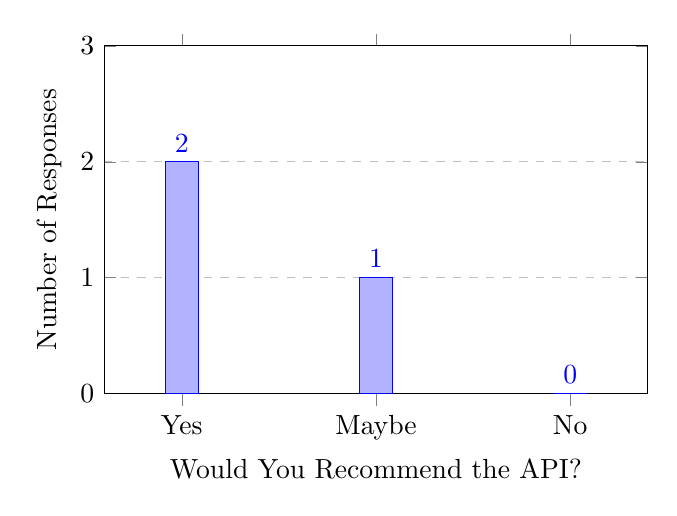
\begin{tikzpicture}
    \begin{axis}[
      ybar,
      bar width=12pt,
      width=0.7\textwidth,
      height=6cm,
      enlarge x limits=0.2,
      ylabel={Number of Responses},
      xlabel={Would You Recommend the API?},
      symbolic x coords={Yes, Maybe, No},
      xtick=data,
      nodes near coords,
      ymin=0, ymax=3,
      ymajorgrids=true,
      grid style=dashed,
      ]
      \addplot coordinates {(Yes,2) (Maybe,1) (No,0)};
    \end{axis}
  \end{tikzpicture}
  \caption{Recommendation Likelihood}
\end{figure}

\subsection{Conclusion}

The solver's API was rated as clear and usable, with minor improvements
suggested for documentation and configurability. All reviewers would recommend
it for use in larger numerical projects, provided additional examples and
higher-level wrappers are included.

\newpage{}

\section{Performance Test Results}
\label{sec:perf-test-results}

\subsection{Raw Runtime Data Table}

\begin{table}[H]
  \centering
  \caption{Runtime measurements for mixed-precision vs. double-precision (10 runs)}
  \begin{tabular}{c|c|c}
    \toprule
    \textbf{Run} & \textbf{Mixed Precision (ms)} & \textbf{Double Precision (ms)} \\
    \midrule
    1      & 11.8                    & 15.4                     \\
    2      & 11.7                    & 15.5                     \\
    3      & 11.6                    & 15.4                     \\
    4      & 11.9                    & 15.3                     \\
    5      & 11.8                    & 15.6                     \\
    6      & 11.7                    & 15.5                     \\
    7      & 11.6                    & 15.4                     \\
    8      & 11.7                    & 15.6                     \\
    9      & 11.8                    & 15.5                     \\
    10     & 11.6                    & 15.5                     \\
    \bottomrule
  \end{tabular}
  \label{tab:perf-raw}
\end{table}

\subsection{Summary Statistics Table}

\begin{table}[H]
  \centering
  \caption{Summary of performance results}
  \begin{tabular}{l|c|c}
    \toprule
    \textbf{Metric}               & \textbf{Mixed Precision} & \textbf{Double Precision} \\
    \midrule
    Average Runtime (ms)    & 11.72              & 15.47               \\
    Standard Deviation (ms) & 0.11               & 0.09                \\
    Measured Gain           & \textbf{24.25\%}         & --                  \\
    \bottomrule
  \end{tabular}
  \label{tab:perf-summary}
\end{table}

\newpage{}

\section{\texttt{PrecondGmres} Implementation Comparison}
\label{sec:textttpr-comp}

This section compares the new \texttt{PrecondGmres} implementation with the prior
research prototype \texttt{gmres\_cond} and \texttt{gmres\_cond2}. The goal is
to highlight improvements in modularity, safety, readability, and type handling.
The comparison focuses on six major dimensions: interface design, memory
management, core algorithm logic, type safety, maintainability, and return
behavior.

\subsection*{Interface Design}

\begin{table}[H]
  \centering
  \renewcommand{\arraystretch}{1.2}
  \begin{tabularx}{\linewidth}{%
    >{\raggedright\arraybackslash}l
    >{\raggedright\arraybackslash}X
    >{\raggedright\arraybackslash}X
    }
    \toprule
    \textbf{Aspect}            & \textbf{Old Implementation}                                                                      & \textbf{New Implementation}                                              \\
    \midrule
    Templating           & Six template parameters (\texttt{ATVPREC}, \texttt{T}, \texttt{FACTPREC}, \texttt{RESPREC}, \texttt{WORKPREC}, \texttt{XPREC}) & Three template parameters constrained via \texttt{Refinable<UF, UW, UR>} \\
    Parameter Style      & Long list of raw pointers interleaved with outputs                                         & Clean API with STL containers and logical parameter order          \\
    Preconditioner Input & Passed as separate pointer arrays                                                          & Encapsulated as class members                                      \\
    Callback for \texttt{A*v}  & \texttt{std::function} passed per call                                                           & Replaced with internal \texttt{MatrixMultiply} + \texttt{QDLDL\_solve} calls   \\
    \bottomrule
  \end{tabularx}
  \caption{Interface Design Comparison}
\end{table}

\subsection*{Memory Management}

\begin{table}[H]
  \centering
  \begin{tabularx}{\linewidth}{%
    >{\raggedright\arraybackslash}l
    >{\raggedright\arraybackslash}X
    >{\raggedright\arraybackslash}X
    }
    \toprule
    \textbf{Aspect}         & \textbf{Old Implementation}                   & \textbf{New Implementation}                             \\
    \midrule
    Memory Handling   & Raw \texttt{new[]}/\texttt{delete[]} for all arrays & Automatic \texttt{std::vector} usage                    \\
    Resource Safety   & Manual cleanup at multiple return paths & RAII via containers ensures exception safety      \\
    Temporary Buffers & All manually allocated and deallocated  & Constructed on-demand and destroyed automatically \\
    \bottomrule
  \end{tabularx}
  \caption{Memory and Resource Management}
\end{table}

\subsection*{Algorithm Structure and Numerical Logic}

\begin{table}[H]
  \centering
  \begin{tabularx}{\linewidth}{%
    >{\raggedright\arraybackslash}l
    >{\raggedright\arraybackslash}X
    >{\raggedright\arraybackslash}X
    }
    \toprule
    \textbf{Aspect}            & \textbf{Old Implementation}                         & \textbf{New Implementation}                                  \\
    \midrule
    Arnoldi Loop         & Inline pointer math with duplicated logic     & Modular functions (\texttt{VectorDot}, \texttt{VectorScale}, etc.) \\
    Reorthogonalization  & Implemented via nested loops manually         & Same logic using modular vector operations             \\
    Givens Rotations     & Explicit array indexing and logic inside loop & Decomposed into reusable transformations               \\
    Residual Computation & Custom residual + norm macros                 & Uses templated \texttt{Dnrm2} and subtraction helpers        \\
    \bottomrule
  \end{tabularx}
  \caption{Numerical Logic and Algorithm Flow}
\end{table}

\subsection*{Precision and Type Handling}

\begin{table}[H]
  \centering
  \begin{tabularx}{\linewidth}{%
    >{\raggedright\arraybackslash}l
    >{\raggedright\arraybackslash}X
    >{\raggedright\arraybackslash}X
    }
    \toprule
    \textbf{Aspect}             & \textbf{Old Implementation}                    & \textbf{New Implementation}                    \\
    \midrule
    Precision Control     & Manual cast between six different types  & Centralized via \texttt{Refinable<UF, UW, UR>} \\
    Casting Overhead      & Frequent \texttt{static\_cast} at use sites    & Type conversions localized and explicit  \\
    Precision Consistency & Developer responsible for type coherence & Enforced via compile-time constraints    \\
    \bottomrule
  \end{tabularx}
  \caption{Precision and Type Safety}
\end{table}

\subsection*{Maintainability and Readability}

\begin{table}[H]
  \centering
  \begin{tabularx}{\linewidth}{%
    >{\raggedright\arraybackslash}l
    >{\raggedright\arraybackslash}X
    >{\raggedright\arraybackslash}X
    }
    \toprule
    \textbf{Aspect}       & \textbf{Old Implementation}                        & \textbf{New Implementation}                       \\
    \midrule
    Function Length & 500+ lines in one function                   & Structured into ~50-line modular components \\
    Naming          & Many temporary or cryptic variable names     & Clear variable names and helper functions   \\
    Readability     & Difficult to trace control flow              & Code reads like algorithm pseudocode        \\
    Extensibility   & Difficult to adapt to new formats or solvers & Designed for modular extension              \\
    \bottomrule
  \end{tabularx}
  \caption{Maintainability and Readability}
\end{table}

\subsection*{Return and Error Handling}

\begin{table}[H]
  \centering
  \begin{tabularx}{\linewidth}{%
    >{\raggedright\arraybackslash}l
    >{\raggedright\arraybackslash}X
    >{\raggedright\arraybackslash}X
    }
    \toprule
    \textbf{Aspect}        & \textbf{Old Implementation}                    & \textbf{New Implementation}                                      \\
    \midrule
    Return Method    & Outputs written to raw pointer arguments & Returns computed vector directly                           \\
    Error Handling   & No explicit error path                   & Returns empty vector on failure (e.g., size mismatch)      \\
    Status Reporting & Total iterations via output reference    & Embedded in solver’s internal state (TBD for next version) \\
    \bottomrule
  \end{tabularx}
  \caption{Return Value and Error Handling}
\end{table}

\subsection*{Summary}

The new \texttt{PrecondGmres} implementation significantly improves over the previous
research prototype in terms of code clarity, modularity, type safety, and
maintainability. By adopting standard C++ constructs and a principled separation
of responsibilities, the solver becomes easier to reason about, extend, and
integrate. The use of constraints through the \texttt{Refinable} concept further
ensures compile-time precision correctness, reducing the risk of errors in
mixed-precision configurations.

\end{document}
